\documentclass[a4paper,12pt]{article}
\usepackage[utf8]{inputenc}
\usepackage{amsmath}
\usepackage{amsfonts}
\usepackage{amssymb}
\usepackage{graphicx}
\usepackage{braket}

\numberwithin{equation}{section}
\renewcommand\thesubsection{\alph{subsection}}
\newcommand{\bvp}[1]{\mathbf{#1}'}
\newcommand{\bv}[1]{\mathbf{#1}}

%opening
\title{Quantum II midterm question}
\author{Vincent Baker}

\begin{document}

\maketitle

\section{Problem 1: ``Graph thing with the lines''}
Recall the lowering operator $L_-\ket{j,\ m}=\sqrt{(j+m)(j-m+1)}\ket{j,\ m-1}$.
The lowering operator is the same for any angular momentum state (orbit, spin or total).\\
The 6 states of an electron with orbital angular momentum 1, spin $\frac{1}{2}$ are shown below.
\\
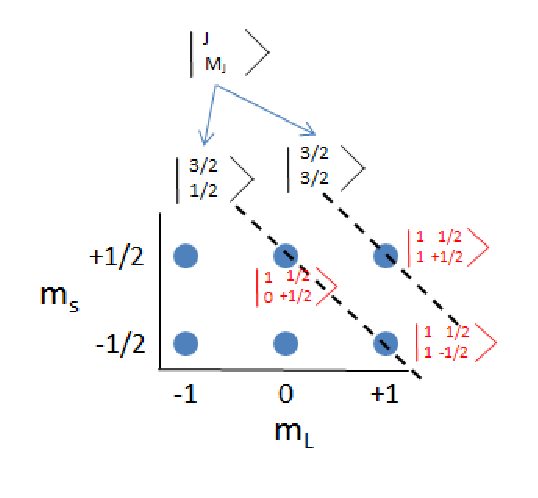
\includegraphics{momentum}
\\
The top-right state $\ket{\substack{\ell\ s\\m_\ell\ m_s}}=\ket{\substack{1\ 1/2\\ 1\ 1/2}}$ 
can be written in the TOTAL angular momentum basis as 
$\ket{\substack{J \\M_J}}=\ket{\substack{3/2 \\ 3/2} }$.\\
a) In the total angular momentum basis apply the lowering operator $J_-$ to the top-right state 
basis to find the next lower state.
\begin{gather}
 J_-\ket{ \substack{3/2 \\ 3/2} } = \alpha\ket{ \substack{3/2 \\ 1/2} }
\end{gather}
\\
b) Also apply the lowering operator $(L_-+S_-)$ to the top-right state in the spin-orbit basis:
\begin{gather}
 (L_-+S_-)\ket{\substack{1\ 1/2\\ 1\ 1/2}}=\beta\ket{\substack{1\\0}\ \substack{1/2\\1/2}}    
 + \gamma\ket{\substack{1\\1}\ \substack{1/2\\-1/2}}
\end{gather}
c) Use 1.1 and 1.2 to write the total angular momentum state $\ket{ \substack{3/2 \\ 1/2} }$ 
as a linear combination of the spin-orbit states $\ket{\substack{1\\0}\ \substack{1/2\\1/2}}$ and $\ket{\substack{1\\1}\ \substack{1/2\\-1/2}}$.

\section{Solution}
a) Applying $J_-$ we find:
\begin{gather}
 J_-\ket{ \substack{3/2 \\ 3/2} } = \sqrt{3}\ket{ \substack{3/2 \\ 1/2} }
\end{gather}
b) Applying $(L_-+S_-)$ we find:
\begin{gather}
 (L_-+S_-)\ket{\substack{1\ 1/2\\ 1\ 1/2}}=\sqrt{2}\ket{\substack{1\\0}\ \substack{1/2\\1/2}}    
 + \sqrt{1}\ket{\substack{1\\1}\ \substack{1/2\\-1/2}}
\end{gather}
c) We can therefore write the total angular momentum state as:
\begin{gather}
 \ket{ \substack{3/2 \\ 1/2} }=\sqrt{\frac{2}{3}}\ket{\substack{1\\0}\ \substack{1/2\\1/2}}    
 + \sqrt{\frac{1}{3}}\ket{\substack{1\\1}\ \substack{1/2\\-1/2}}
\end{gather}

\end{document}
